\documentclass[a4paper, 11pt]{report}% autres choix : book, report
\usepackage[utf8]{inputenc}% gestion des accents (source)
\usepackage[T1]{fontenc}% gestion des accents (PDF)
\usepackage[francais]{babel}% gestion du français
\usepackage{natbib}% utilisation du lib de référence zotero
\usepackage{textcomp}% caractères additionnels
\usepackage{mathtools,amssymb,amsthm}% packages de l'AMS + mathtools
\usepackage{lmodern}% police de caractère
\usepackage{geometry}% gestion des marges
\usepackage{graphicx}% gestion des images
\usepackage{xcolor}% gestion des couleurs
\usepackage{array}% gestion améliorée des tableaux
\usepackage{calc}% syntaxe naurelle pour les calculs
\usepackage{titlesec}% pour les sections
\usepackage{titletoc}% pour la table des matières
\usepackage{fancyhdr}% pour les en-têtes
\usepackage{titling}% pour le titre
\usepackage{enumitem}% pour les listes numérotées
\usepackage[hyphens]{url} % Pour des césures correctes dansles URLs
\usepackage[pdfauthor = {{MB TC AP}}, pdftitle = {{Modelisation Lokta Volterra}}, pdfstartview = Fit, pdfpagelayout = SinglePage , pdfnewwindow = true, bookmarksnumbered = true, breaklinks, colorlinks, linkcolor = black, urlcolor = black, citecolor = cyan, linktoc = all]{hyperref}
\usepackage{titlesec}

\titleformat{\chapter}[block]
  {\normalfont\Huge\bfseries}% font of number
  {\thechapter~ -}% format of number
  {20pt}% space between number and title
  {\Huge}% font of title
  
% Taille des marges
\geometry{hmargin=2.8cm,vmargin=2.8cm}

% RAZ des numéros de section après un chapitre
\makeatletter\@addtoreset{section}{chapter}\makeatother
% Pour mettre des I, II, etc. aux parties
\renewcommand{\thepart}{\Roman{part}}
% Pour mettre des 1, 2, etc. aux chapitres
\renewcommand{\thechapter}{\Roman{chapter}}
% Idem pour les sections et avoir le numéro de chapitre
\renewcommand{\thesection}{\Roman{section}}
% Idem pour les sous-sections et avoir le numéro de chapitre
\renewcommand{\thesubsection}{\Roman{section}.\arabic{subsection}}

\titlecontents{section}%
	[1.5em]% retrait à gauche
	{\addvspace{1em plus 0pt}\bfseries}% matériel avantcommun aux entrées numérotées ou pas
	{\contentslabel{2em}}% avant lorsqu'il y a un numéro
	{\hspace{-1.3em}}% avant lorsqu'il n'y a pas de numéro
	{\hfill\contentspage}% points de suspension et no page
	[\addvspace{0pt}]% matériel après
	
	\dottedcontents{subsection}%
	[3em]% retrait gauche
	{\addvspace{0pt}}% matériel avant
	{1.5em}% espacement de contentslabel
	{0.75em}% espace entre les . . . .
    [\addvspace{0pt}]% matériel après

    \dottedcontents{subsubsection}%
	[4.5em]% retrait gauche
	{\addvspace{0pt}}% matériel avant
	{1.5em}% espacement de contentslabel
	{0.75em}% espace entre les . . . .
    [\addvspace{0pt}]% matériel après

% En-tête, pied de page
\pagestyle{fancy}
\fancyhead[O]{Mini-Pojet \\Lokta Volterra}
\fancyhead[R]{Modélisation ST2}
\fancyhead[L]{
\includegraphics[height=1cm]{images/cs.png}}

\renewcommand{\footrulewidth}{1pt}
\fancyfoot[C]{\thepage}
\fancyfoot[R]{Matthieu BRIET \\Tanguy COLLEVILLE \\ Antoine PAGNEUX}
\fancyfoot[L]{Groupe 218}
    

\begin{document}
    % Page de Garde
    \begin{titlepage}
        \newcommand{\HRule}{\rule{\linewidth}{0.5mm}}
        \begin{center}
            % En-têtes
            \textsc{\LARGE{} Mini-Projet Modélisation} \\[0.5cm] 
            \textsc{\Large{} CentraleSupélec - 1A} \\[0.5cm]
            \textsc{\large{} Groupe 218} \\[0.5cm] 
            % Titre
            \HRule \\[0.6cm]
            {\huge\bfseries{} Lokta Volterra} \\[0.25cm]
            \HRule \\[1.5cm]
            % Date
            {\large\today} \\[2cm] 
            % Logo CS
            
\includegraphics[width=8cm]{images/cs.png}
            \\[2cm] 
        \end{center}
        \vfill{}
        % Auteurs
        \begin{minipage}{0.45\linewidth}
            \begin{flushleft}
                \Large\textit{Auteurs :} \\
                Matthieu \textsc{BRIET} \\
                Tanguy \textsc{COLLEVILLE} \\
                Antoine \textsc{PAGNEUX} 
            \end{flushleft}
        \end{minipage}
    \end{titlepage}

    % Table des matières
    \tableofcontents
    % Table des figures
    \listoffigures
    % Table des tableaux
    %\listoftables

    \newpage
    \section{Introduction}
        \subsection{blabla}
        L'objectif de ce projet de modélisation est de proposer une simulation de l'évolution des populations,  
        d'un couple proie prédateur dans un écosystème, par le biais des équations de Lotka Volterra. Dans un premier temps,
        Nous étudirons et developperons  le modèle à temps continu pour ensuite nous intéresser à la modélisation
        en temps discret. Nous nous interesserons à l'évolution des populations de sardines et de requins
        dans la mer adriatique. Ce type d'étude peut aider des états à prendre des mesures politiques environnementales 
        et commerciale afin de préserver les écosystèmes des impacts de l'activité humaine, telle que la pêche intensive
        qui menace certaines espèces. 
        \subsection{blabla}

    \section{Modélisation à état continu}
        \subsection{Mise en équation du modèle Lotka Volterra}
        % description équation formulation du problème de Cauchy + Schéma d'Euler avec convergence du modèle prouvé 
        On note $u$ la densité de proies et $v$ la densité de prédateurs. On note ensuite $w$ l'effort de pêche. On cherche à connaître en l'évolution de ces trois grandeurs au cours du temps\
        Ces grandeurs vérifient le système d'équations différentielles non linéaires suivant : 
        $ \left\{
            \begin{array}[t]{l}
                \dfrac{u}{t} = \left( a_1 - b_1 u - \dfrac{c_1 v}{u+ k_1}  \right) u - mquw \\
                \dfrac{v}{t} = \left( a_2 - \dfrac{c_2 v}{u+ k_2} \right) v \\
                \dfrac{w}{t} = \lambda \left( pmqu - c \right) w
            \end{array}
        \right.$
        Avec les conditions initiales suivantes :  $u(0) \geq 0$, $v(0) \geq 0$ et $w(0) \geq 0$.
        On en déduit le schéma d'euler explicite suivant : 
        $ \left\{
            \begin{array}[t]{l}
                u_{n+1} = u_n + h \left( \left( a_1 - b_1 u_n - \dfrac{c_1 v_n}{u_n + k_1}  \right) u_n - mqu_n w_n \right)\\
                v_{n+1} = v_n + h \left( \left( a_2 - \dfrac{c_2 v_n}{u_n + k_2} \right) v_n \right\\
                w_{n+1} = w_n + h \left( \lambda \left( pmq u_n - c \right) w_n \right)
            \end{array}
        \right.$
        Ce système est convergent d'ordre 1.

        %copie d'analyse des points d'equ
        \subsection{Analyse des points d'équililbre}
        $ \left\{
            \begin{array}[t]{l}
                \dfrac{u}{t} =0 \\
                \dfrac{v}{t} = 0\\
                \dfrac{w}{t} = 0
            \end{array}
        \right.$
        
        %Courbes : Comparaison Scipy / Euler avec 3 courbes et val eq 
        \subsection{Evolution des grandeurs ...}
        \begin{center}
            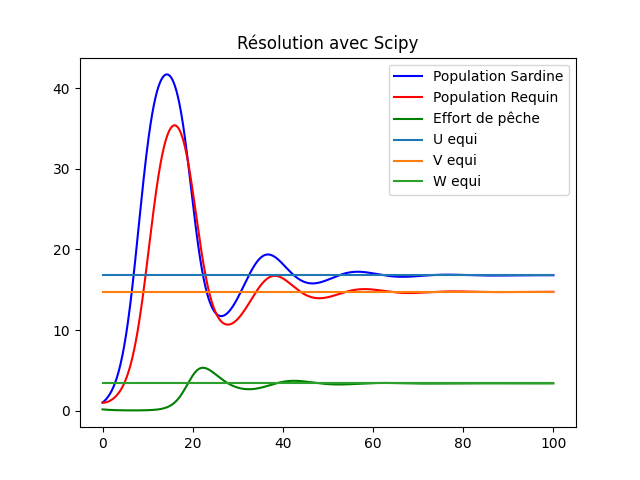
\includegraphics[width=10cm]{figures/Scipy_good_conditions.png}
            \captionof{figure}{Evolution des grandeurs, méthode Scipy}
        \end{center}

        \begin{center}
            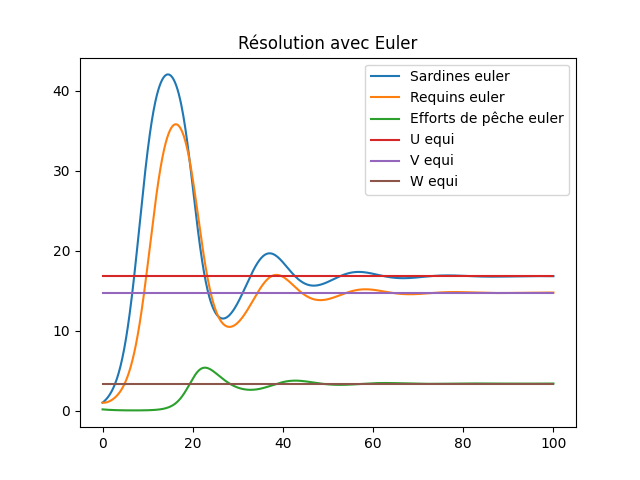
\includegraphics[width=10cm]{figures/Euler_good_conditions.png}
            \captionof{figure}{Evolution des grandeurs, méthode d'Euler}
        \end{center}

        \begin{center}
            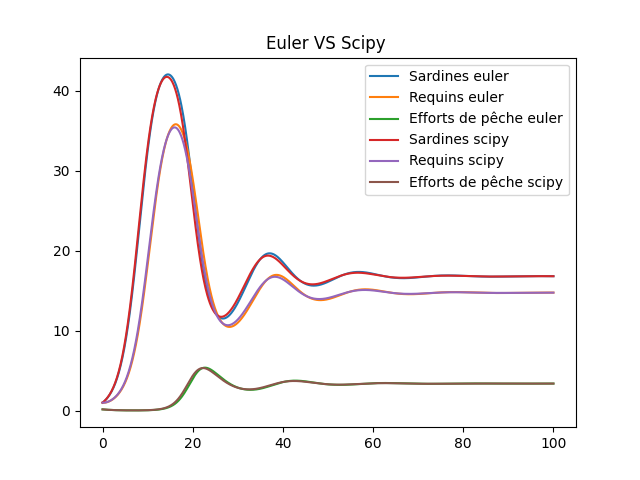
\includegraphics[width=10cm]{figures/Euler_VS_Scipy_good_conditions.png}
            \captionof{figure}{Comparaison des méthodes de résolution avec Euler explicite et Scipy}
        \end{center}

        % Courbes  : 3 portraits de phase 2d + ligne 3D u,v,w 
        \subsection{Portrait de phase des grandeurs $u,v,w$}
        \begin{center}
            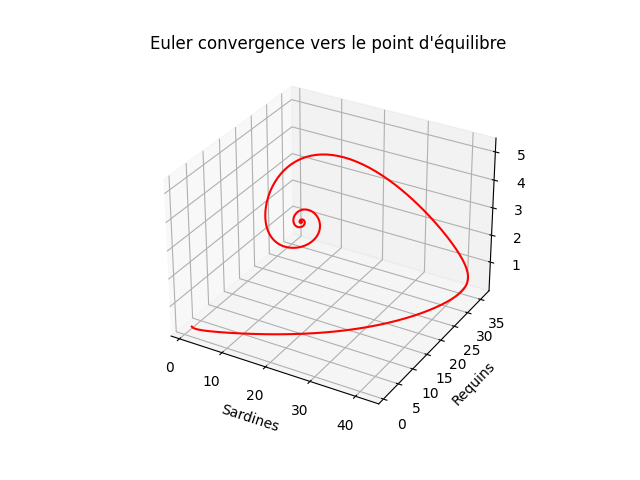
\includegraphics[width=10cm]{figures/convergence_3d_point_equilibre.png}
            \captionof{figure}{Convergence vers le point d'équilibre}
        \end{center}

        \begin{center}
            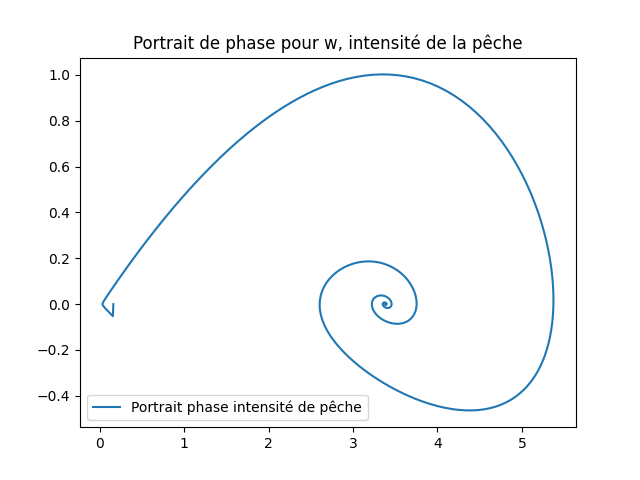
\includegraphics[width=10cm]{figures/Portrait_de_phase_peche.png}
            \captionof{figure}{Portrait de phase de l'effort de peche}
        \end{center}

        \begin{center}
            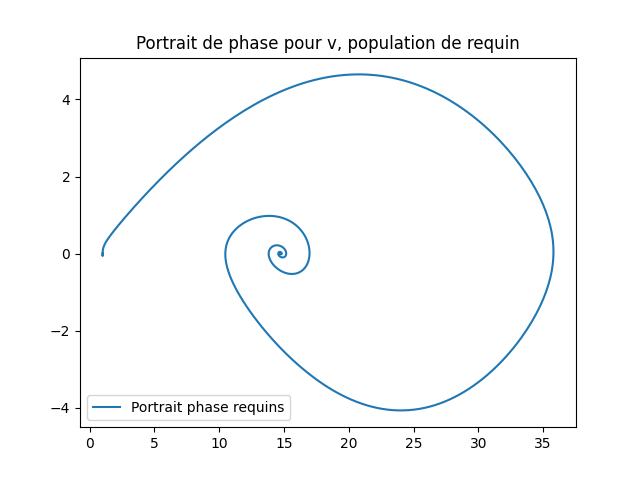
\includegraphics[width=10cm]{figures/Portrait_de_phase_requins.png}
            \captionof{figure}{Portrait de phase de la densité de requins}
        \end{center}

        \begin{center}
            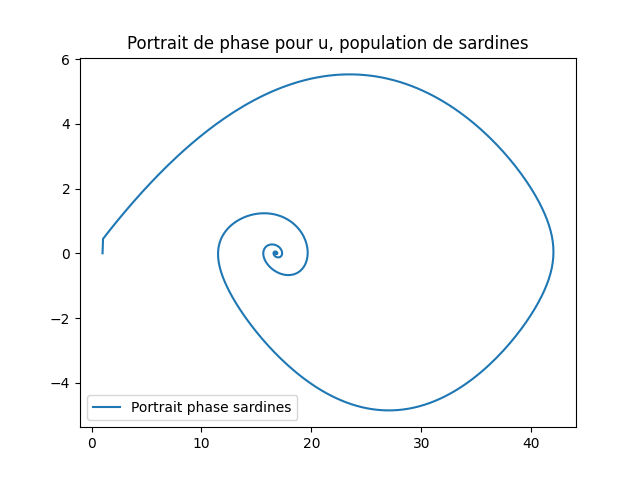
\includegraphics[width=10cm]{figures/Portrait_de_phase_sardine.png}
            \captionof{figure}{Portrait de phase de la densité de sardines}
        \end{center}

        % comparasion à nos attentes dans la vie réelle --> regarder les sardines disparaissent mer adriatique
        \subsection{Conclusion}

        % on prends l'exemple y'a que des sardines pas de prédateurs 
        \subsection{Cas particulier du système sans prédateur}

    \section{Modélisation à événements discrets}
        \subsection{blabla}
        % Réseau de pétri 

    \nocite{*}
    \bibliographystyle{plain}
    \bibliography{lib}
\end{document}